
\documentclass{beamer}
\usepackage[utf8]{inputenc}
\usepackage{url}
\usepackage{algorithm}
\usepackage{algpseudocode}
\usepackage{lmodern}
\usepackage{natbib}
\usepackage{tikz}
\usepackage{physics}
\usepackage{graphicx} % Allows including images
\graphicspath{ {./images/} }
\usepackage{booktabs} % Allows the use of \toprule, \midrule and \bottomrule in tables
\usepackage{tikz}
\usetikzlibrary{arrows.meta}


\usetikzlibrary{mindmap, trees, shadows, shapes, calc, fadings, positioning, decorations.pathreplacing, intersections, shapes, arrows}

%\usetheme{Hannover}
%\usecolortheme{spruce}
% EPIC FAIL
\usetheme{default}
%\usecolortheme{beetle}
\usepackage{graphics}

\usepackage{color}
\definecolor{new_turquoise}{RGB}{40,151,158}%{251,190,94}
\setbeamercolor{title}{fg=new_turquoise}


%\usepackage[colorlinks=true, urlcolor=blue, linkcolor=red]{hyperref}


\makeatletter
\setbeamertemplate{frametitle}{
    \ifbeamercolorempty[bg]{frametitle}{}{\nointerlineskip}%
    \@tempdima=\textwidth%
    \advance\@tempdima by\beamer@leftmargin%
    \advance\@tempdima by\beamer@rightmargin%
    \vspace*{0.8cm} 
    %\hspace*{-3cm}
    %%%%%%%%%%%%% For example insert shift to right
    \begin{beamercolorbox}[sep=0.3cm,center,wd=\the\@tempdima]{frametitle}
        \usebeamerfont{frametitle}%
        \vbox{}\vskip-1ex%
        \if@tempswa\else\csname beamer@ftecenter\endcsname\fi%
        \strut\insertframetitle\strut\par%
        {%
            \ifx\insertframesubtitle\@empty%
            \else%
            {\usebeamerfont{framesubtitle}\usebeamercolor[fg]{framesubtitle}\insertframesubtitle\strut\par}%
            \fi
        }%
        \vskip-1ex%
        \if@tempswa\else\vskip-.3cm\fi% set inside beamercolorbox... evil here...
    \end{beamercolorbox}%
}
\makeatother

\setbeamercolor{frametitle}{fg=new_turquoise}
\setbeamertemplate{itemize item}{\color{new_turquoise}$\blacksquare$}
\setbeamertemplate{itemize subitem}{\color{new_turquoise}$\blacksquare$}


% --- ENUMERATE ITEMS ---
\setbeamertemplate{enumerate item}{\color{new_turquoise}\insertenumlabel}
\setbeamertemplate{enumerate subitem}{\color{new_turquoise}\insertsubenumlabel}

\setbeamertemplate{caption}{\raggedright\insertcaption\par}

% --- COLOR THE TABLE OF CONTENTS ENTRIES ---
\setbeamercolor{section in toc}{fg=new_turquoise}
\setbeamercolor{subsection in toc}{fg=new_turquoise}
\setbeamercolor{subsubsection in toc}{fg=new_turquoise}



\usebackgroundtemplate{
    \includegraphics[width=\paperwidth,height=\paperheight]{figs/slide-title.jpg}
} 

\title{\fontsize{49}{7.2}{\bf Fundamental Algorithmic Techniques VII}}
%\author{JW}
\date{\color{new_turquoise}\today}
%S\titlegraphic{\includegraphics[width=2cm]{figs/jw.png}}

\begin{document}
\frame{\titlepage}
%% SLIDE 1 - INTRO TO THE TEAM
%%%%%%%%%%%%%%%%%%%%%%%%%%%%%%%%%%%%%%%%%%%%%%%%%%%%%

\usebackgroundtemplate{
    \includegraphics[width=\paperwidth,height=\paperheight]{figs/slide-pages}
} 


\setbeamertemplate{subsection in toc}{
  \color{new_turquoise}$\blacksquare$\color{black}~~\inserttocsubsection
}


% Outline frame
\begin{frame}{Outline}
    \tableofcontents
\end{frame}



\section{Graphs Introduction}
%\begin{frame}{Graph: Oldest Application}
%\end{frame}

\begin{frame}{Graphs: Oldest Application}
  \textit{Early applications of graphs in historical contexts...}
  
  \vspace{1em}
  
  \begin{columns}[T, onlytextwidth]
    \begin{column}{0.48\textwidth}
      \centering
      \includegraphics[width=.75\textwidth]{Algos_figs/family-tree-of-the-capetians.jpg}\\
      \small Capetian dynasty
    \end{column}
    \hfill
    \begin{column}{0.48\textwidth}
      \centering
      \includegraphics[width=\textwidth]{Algos_figs/To26754wHyk.jpg}\\
      \small Kazakh Clans
    \end{column}
  \end{columns}
\end{frame}


\begin{frame}{Introduction to Graphs: Basic Definitions}

  \centering
  \begin{columns}[T, onlytextwidth]
    \begin{column}{0.4\textwidth}
      \centering
      \includegraphics[width=\textwidth]{Algos_figs/GraphStructure.png}
      \par\small %Structure
    \end{column}
    \hfill
    \begin{column}{0.4\textwidth}
      \centering
      \includegraphics[width=\textwidth]{Algos_figs/Tree_Graph.jpeg}
      \par\small Tree \& graph
    \end{column}
  \end{columns}

\small
  \begin{block}{\color{new_turquoise}Formal Definition}
    A (simple) graph is a pair of sets $(V, E)$, where:
    \begin{itemize}
    \item $V$ is a non-empty finite set of \textbf{vertices} (or \textbf{nodes}),
      \item $E$ is a set of pairs of elements from $V$, called \textbf{edges}.
    \end{itemize}
  \end{block}

  %\vspace{1em}

  \begin{description}
    \item[\color{new_turquoise}Undirected graph:] Edges are unordered pairs (2-element sets).  
    We write $uv$ (or $\{u,v\}$) for the edge between $u$ and $v$.

    \item[\color{new_turquoise}Directed graph:] Edges are ordered pairs.  \\
    We write $u \to v$ (or $(u,v)$) for the edge $u$ to $v$.
  \end{description}

\end{frame}






\section{Data Structures for Graphs}

\begin{frame}{Graph Basics: Subgraphs, Walks, and Connectivity}


  \textcolor{new_turquoise}{Subgraph:} $G' = (V', E')$ is a subgraph of $G = (V, E)$ if $V' \subseteq V$ and $E' \subseteq E$.  
  %\textit{Proper subgraph}: any subgraph $\neq G$.

  \medskip

  \textcolor{new_turquoise}{Walk:} sequence of vertices where consecutive vertices are adjacent.  
\medskip

  \textcolor{new_turquoise}{Path:} a walk with no repeated vertices.
\medskip

  \textcolor{new_turquoise}{Reachable:} $v$ is reachable from $u$ if a path exists between them.
\medskip

  \textcolor{new_turquoise}{Connected:} every pair of vertices is reachable.
\medskip

  \textcolor{new_turquoise}{Component:} maximal connected subgraph.


\end{frame}




\begin{frame}{Trees, Forests, and Spanning Subgraphs}

\textcolor{new_turquoise}{Closed walk:} starts and ends at same vertex.\\
\medskip 
\textcolor{new_turquoise}{Cycle:} closed walk with no repeated vertices (except start/end).\\
\medskip
\textcolor{new_turquoise}{Acyclic graph:} contains no cycles → called a \textcolor{new_turquoise}{forest}.\\
\medskip 
\textcolor{new_turquoise}{Tree:} connected acyclic graph (i.e., one-component forest).\\
\medskip
\textcolor{new_turquoise}{Spanning tree:} subgraph that is a tree and includes \textbf{all} vertices of $G$.\\
\medskip
$G$ has a spanning tree $\iff$ $G$ is \textcolor{new_turquoise}{connected}.\\
\medskip
\textcolor{new_turquoise}{Spanning forest:} spanning tree for each component.
\end{frame}




\begin{frame}{Directed Graphs: Walks, Reachability, and DAGs}

\textcolor{new_turquoise}{Directed walk:} $v_0 \to v_1 \to \cdots \to v_\ell$ where each $(v_{i-1}, v_i) \in E$.\\

\textcolor{new_turquoise}{Directed path/cycle:} no repeated vertices (except start/end in cycle). \\

$v$ is \textcolor{new_turquoise}{reachable} from $u$ if a directed path $u \leadsto v$ exists. \\

\textcolor{new_turquoise}{Strongly connected:} every vertex reachable from every other. \\

\textcolor{new_turquoise}{Directed Acyclic Graph (DAG):} no directed cycles.

\vspace{1.5em}

\centering
\begin{columns}[T, onlytextwidth]
  \begin{column}{0.45\textwidth}
    \centering
    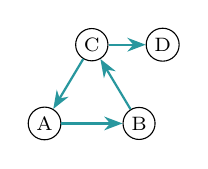
\begin{tikzpicture}[>={Stealth}, every node/.style={circle, draw, inner sep=1.5pt, fill=white, font=\scriptsize}]
      \node (A) at (0,0) {A};
      \node (B) at (1.2,0) {B};
      \node (C) at (0.6,1) {C};
      \node (D) at (1.5,1) {D};
      \draw[->, new_turquoise, thick] (A) -- (B);
      \draw[->, new_turquoise, thick] (B) -- (C);
      \draw[->, new_turquoise, thick] (C) -- (A); % cycle
      \draw[->, new_turquoise, thick] (C) -- (D);
    \end{tikzpicture}
    \par\small\textcolor{new_turquoise}{Cyclic digraph}
  \end{column}
  \hfill
  \begin{column}{0.45\textwidth}
    \centering
    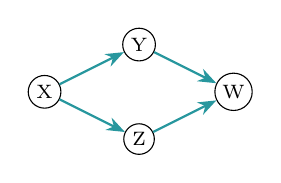
\begin{tikzpicture}[>={Stealth}, every node/.style={circle, draw, inner sep=1.5pt, fill=white, font=\scriptsize}]
      \node (X) at (0,0) {X};
      \node (Y) at (1.2,0.6) {Y};
      \node (Z) at (1.2,-0.6) {Z};
      \node (W) at (2.4,0) {W};
      \draw[->, new_turquoise, thick] (X) -- (Y);
      \draw[->, new_turquoise, thick] (X) -- (Z);
      \draw[->, new_turquoise, thick] (Y) -- (W);
      \draw[->, new_turquoise, thick] (Z) -- (W);
      % No back edges → acyclic
    \end{tikzpicture}
    \par\small\textcolor{new_turquoise}{DAG (acyclic)}
  \end{column}
\end{columns}

\end{frame}


\begin{frame}{Directed Graphs: Walks, Reachability, Weighted \& DAGs}
\small

\textcolor{new_turquoise}{Directed walk:} $v_0 \to v_1 \to \cdots \to v_\ell$ where each $(v_{i-1}, v_i) \in E$.\\
\textcolor{new_turquoise}{Directed path/cycle:} no repeated vertices (except start/end in cycle). \\
$v$ is \textcolor{new_turquoise}{reachable} from $u$ if a directed path $u \leadsto v$ exists. \\
\textcolor{new_turquoise}{Strongly connected:} every vertex reachable from every other. \\
\textcolor{new_turquoise}{Directed Acyclic Graph (DAG):} no directed cycles. \\[0.8em]

\textcolor{new_turquoise}{Unweighted graph:} edges have no numerical values. \\
\textcolor{new_turquoise}{Weighted graph:} each edge $(u,v)$ has a weight $w(u,v) \in \mathbb{R}$. \\[0.5em]

For vertex $v$: \quad
$\deg^-(v) = |\{u : (u,v) \in E\}|$ \textcolor{new_turquoise}{(in-degree)}, \quad
$\deg^+(v) = |\{u : (v,u) \in E\}|$ \textcolor{new_turquoise}{(out-degree)}.

\vspace{1em}

\centering
\begin{columns}[T, onlytextwidth]
  \begin{column}{0.45\textwidth}
    \centering
    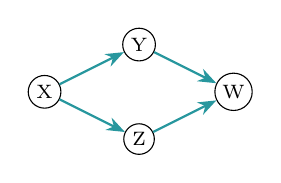
\begin{tikzpicture}[>={Stealth}, every node/.style={circle, draw, inner sep=1.5pt, fill=white, font=\scriptsize}]
      \node (X) at (0,0) {X};
      \node (Y) at (1.2,0.6) {Y};
      \node (Z) at (1.2,-0.6) {Z};
      \node (W) at (2.4,0) {W};
      \draw[->, new_turquoise, thick] (X) -- (Y);
      \draw[->, new_turquoise, thick] (X) -- (Z);
      \draw[->, new_turquoise, thick] (Y) -- (W);
      \draw[->, new_turquoise, thick] (Z) -- (W);
    \end{tikzpicture}
    \par\small\textcolor{new_turquoise}{DAG (acyclic)}
  \end{column}
  \hfill
  \begin{column}{0.45\textwidth}
    \centering
    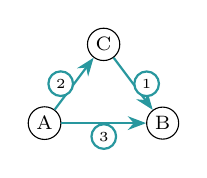
\begin{tikzpicture}[>={Stealth}, every node/.style={circle, draw, inner sep=1.5pt, fill=white, font=\scriptsize}]
      \node (A) at (0,0) {A};
      \node (B) at (1.5,0) {B};
      \node (C) at (0.75,1) {C};
      \draw[->, new_turquoise, thick] (A) -- (B) node[midway, below, font=\tiny, text=black] {3};
      \draw[->, new_turquoise, thick] (A) -- (C) node[midway, left, font=\tiny, text=black] {2};
      \draw[->, new_turquoise, thick] (C) -- (B) node[midway, right, font=\tiny, text=black] {1};
    \end{tikzpicture}
    \par\small\textcolor{new_turquoise}{Weighted digraph}
  \end{column}
\end{columns}

\end{frame}



\section{Graph Representations}
\begin{frame}{Graphs Representations: Adjacency Matrix}

  \centering
  \begin{columns}[T, onlytextwidth]
    \begin{column}{0.48\textwidth}
      \centering
      \includegraphics[width=\textwidth]{Algos_figs/adjmatrixundirected.png}
      \par\small Undirected graph \\ (symmetric matrix)
    \end{column}
    \hfill
    \begin{column}{0.48\textwidth}
      \centering
      \includegraphics[width=\textwidth]{Algos_figs/adjmatrixdirected.png}
      \par\small Directed graph \\ (asymmetric matrix)
    \end{column}
  \end{columns}

  \vspace{1em}
  \footnotesize
  \textit{Adjacency matrices use $\mathcal{O}(V^2)$ space. \\
  Efficient for dense graphs but obvious waste of memory for sparse.} \\ 
\medskip

  $\Rightarrow$ \textcolor{new_turquoise}{Sparse Matrices}
\end{frame}


\begin{frame}{Graphs Representations: Sparse Matrix Representations}
\footnotesize
Sparse matrices store only non-zero values to save space. Three standard formats of size $\mathcal{O}(V_{non\, zero})$:

\vspace{1em}

\begin{columns}[T, onlytextwidth]
  \begin{column}{0.32\textwidth}
    \centering
    \textcolor{new_turquoise}{COO (Coordinate List)}\\
    \smallskip
    Store triplets: (row, col, value)\\
    \smallskip
    \begin{tabular}{|c|c|c|}
      \hline
      i & j & val \\ \hline
      0 & 2 & 5 \\
      1 & 0 & 3 \\
      2 & 2 & 7 \\ \hline
    \end{tabular}
    \par\small Unsorted; simple to build
  \end{column}
  \hfill
  \begin{column}{0.32\textwidth}
    \centering
    \textcolor{new_turquoise}{CSR (Compressed Sparse Row)}\\
    \smallskip
    \texttt{values}: {[5,3,7]}\\
    \texttt{col\_idx}: {[2,0,2]}\\
    \texttt{row\_ptr}: {[0,1,2,3]}
    \par\small Efficient row access; used for vector multiplication
  \end{column}
  \hfill
  \begin{column}{0.32\textwidth}
    \centering
    \textcolor{new_turquoise}{CSC (Compressed Sparse Column)}\\
    \smallskip
    \texttt{values}: {[3,5,7]}\\
    \texttt{row\_idx}: {[1,0,2]}\\
    \texttt{col\_ptr}: {[0,1,1,3]}
    \par\small Efficient column access; transpose of CSR
  \end{column}
\end{columns}

\vspace{1em}
{\footnotesize
\textit{COO = easy construction; CSR/CSC = efficient computation}}
\end{frame}


\section{Graph Operations}


\begin{frame}{Graphs: Basic Operations}
  Common operations on graph data structures:
  
  \vspace{1em}
  
  \begin{description}
    \item[\textcolor{new_turquoise}{\texttt{add\_vertex(G, x)}}] Inserts a new vertex $x$ into graph $G$.
    \item[\textcolor{new_turquoise}{\texttt{remove\_vertex(G, x)}}] Removes vertex $x$ and all its incident edges.
    
    \item[\textcolor{new_turquoise}{\texttt{add\_edge(G, x, y)}}] Adds an edge between vertices $x$ and $y$.
    \item[\textcolor{new_turquoise}{\texttt{remove\_edge(G, x, y)}}] Removes the edge between $x$ and $y$.
    
    \item[\textcolor{new_turquoise}{\texttt{adjacent(G, x, y)}}] Returns \texttt{true} if edge $(x,y)$ exists.
    \item[\textcolor{new_turquoise}{\texttt{neighbors(G, x)}}] Returns list of vertices adjacent to $x$.
    
    \item[\textcolor{new_turquoise}{\texttt{get\_vertex\_value(G, x)}}] Retrieves the value stored at vertex $x$.
    \item[\textcolor{new_turquoise}{\texttt{set\_vertex\_value(G, x, v)}}] Sets the value of vertex $x$ to $v$.
  \end{description}
  
  \vspace{0.5em}

\end{frame}



\begin{frame}{Graphs: Construction Operations}
  Operations to combine or transform graphs:
  
  \vspace{1em}
  
  \begin{description}
    \item[\textcolor{new_turquoise}{Graph Union}] Creates a new graph by combining two existing graphs $G_1$ and $G_2$.  
    The most common method is the \textit{disjoint union}, which keeps all vertices and edges from both graphs.
    
    \item[\textcolor{new_turquoise}{Graph Intersection}] Creates a new graph containing only the vertices and edges that are common to both $G_1$ and $G_2$.
    
    \item[\textcolor{new_turquoise}{Graph Join}] Creates a new graph by adding all possible edges that connect a vertex from $G_1$ to a vertex in $G_2$.
  \end{description}
\end{frame}


\section{Graphs Analysis}

\begin{frame}{Traversal and Analysis Operations}
  Key algorithms for exploring and analyzing graph structure:
  
  \vspace{1em}
  
  \begin{description}
    \item[\textcolor{new_turquoise}{Graph Traversal}] Involves visiting every vertex in the graph.  
    Common algorithms: Depth-First Search (DFS) and Breadth-First Search (BFS).
    
    \item[\textcolor{new_turquoise}{Shortest Path}] Finds the path with minimum total weight between two vertices in a weighted graph.  
    Algorithms: Dijkstra’s, Bellman-Ford, or Floyd–Warshall.
    
    \item[\textcolor{new_turquoise}{Connectivity}] Determines whether the graph is connected (undirected) or strongly/weakly connected (directed), and identifies connected components.
    
    \item[\textcolor{new_turquoise}{Topological Sort}] Arranges vertices of a directed acyclic graph (DAG) in linear order such that for every edge $u \to v$, $u$ comes before $v$.  
    Used in scheduling, build systems, and dependency resolution.
  \end{description}
\end{frame}



%\section{Graph Traversal: Searches}
\begin{frame}{Depth-First Search vs Breadth-First Search}
  % Shared image at the top
  \centering
  \includegraphics[width=0.85\textwidth]{Algos_figs/depth-breadth-first.png}
  \vspace{1.2em}
  % Two columns for descriptions
  \begin{columns}[T, onlytextwidth]
    \begin{column}{0.48\textwidth}
        \centering
      \textcolor{new_turquoise}{\textbf{Breadth-First Search (BFS)}}
      \begin{itemize}
        \item Explores all neighbors at the present depth before moving deeper.
        \item Uses a \textbf{queue} (FIFO).
        %\item Good for: shortest paths (unweighted), level-order traversal.
        %\item Time: $O(V + E)$
      \end{itemize}
    \end{column}
    \hfill
    \begin{column}{0.48\textwidth}
          \centering
      \textcolor{new_turquoise}{\textbf{Depth-First Search (DFS)}}
      \begin{itemize}
        \item Explores as far as possible along each branch before backtracking.
        \item Uses a \textbf{stack} (recursion or explicit LIFO).
      \end{itemize}
    \end{column}
  \end{columns}
\end{frame}

\end{document}
